\chapter{Progettazione}

In questo capitolo viene descritta in maniera maggiormente dettagliata l'architettura del progetto e le scelte che hanno portato alla sua realizzazione.

\section{Progettazione generale del sistema}

Il progetto è stato diviso in tre macro parti e in diverse sottoparti: 
\begin{itemize}
	\item Una parte in esecuzione su un sistema embedded, suddiviso in:
	\begin{itemize}
		\item Rilevamento illuminazione ambientale con il sensore di luce
		\item Rilevamento presenza di automobili con i sensori di prossimità
		\item L'illuminazione di ogni singolo lampione in base alle politiche locali 
		\item Il programma principale che gestisce il web server REST e l'invio delle statistiche al server
	\end{itemize}
	\item Un web server accessibile dagli addetti ai lavori per permettere di leggere e modificare le policy dei singoli lampioni
	\item Una parte in esecuzione su un server che ??
\end{itemize}

Altre info qui.

\section{Architettura complessiva}

yes

TODO class diagram Raspberry Pi

\section{Raspberry Pi architettura REST}
TODO

\section{Policy del sistema}
L'eventuale illuminazione di un lampione è regolata da policy decise a priori e modificabili anche durante l'esecuzione del sistema.
A meno della rilevazione del passaggio di un'auto o di un livello di intensità luminosa eccedente il limite impostato nelle policy, l'unico fattore che viene usato per l'illuminazione è l'orario corrente.

\subsection{Macchina a stati finiti}
Per mostrare il comportamento del sistema riguardante le policy temporali si è utilizzata la macchina a stati finiti semplificata di figura \ref{FSM POLICY}.
Inizialmente i lampioni partono dallo stato "off" e se l'orario corrente (rappresentato dalla variabile t) è successivo all'orario impostato per la policy on, allora il lampione passerà allo stato "on". In seguito quando l'orario supererà la soglia di policy energy on, il lampione andrà in modalità risparmio energetico passando allo stato "energy saving".
Alla fine del periodo di risparmio energetico, impostato da policy energy off, il lampione tornerà allo stato di partenza spegnendosi.

\begin{figure}[ht]
	\centering
	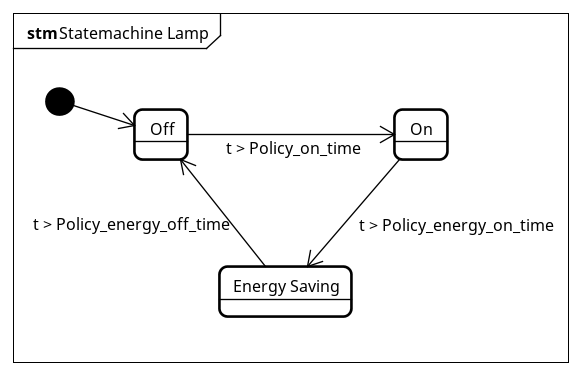
\includegraphics[scale=.8]{figure/Statemachine_Lamp.png}
	\caption{Finished State Machine relativo alle policy del sistema \label{FSM POLICY}}
\end{figure}
\newpage

\section{Controllo presenza auto}
Questa parte si occupa di controllare la presenza di eventuali auto in transito. Utilizzando un sensore di prossimità periodicamente viene calcolata la distanza tra il sensore e l'ostacolo più vicino per valutare se un'auto possa essere in transito in quel momento sulla carreggiata.

\subsection{Comportamento sensore di prossimità}
Per la rappresentazione dell'architettura è stato scelto di utilizzare una Finished State Machine.
Come si può notare in figura \ref{FSM CAR} all'avvio dell'ultrasonic vengono creati due thread concorrenti. Il primo ha il compito di aggiungere e rimuovere i lampioni interessati ad essere notificati del passaggio di auto.
Il secondo invece si occupa di fare la rilevazione della distanza tra il sensore e l'oggetto in quel momento più vicino. Partendo dallo stato "waiting", se è presente almeno un attore, viene effettuata una lettura di distanza e, se il valore è maggiore di 1 metro, aspetta 200 millisecondi per poi tornare nello stato "waiting". Se invece il valore è minore di 1 metro significa che è stata rilevata un auto e quindi vengono notificati tutti i lampioni attualmente in lista. Dopo aver aspettato 5 secondi torna allo stato iniziale di "waiting".


\begin{figure}[tbp]
	\centering
	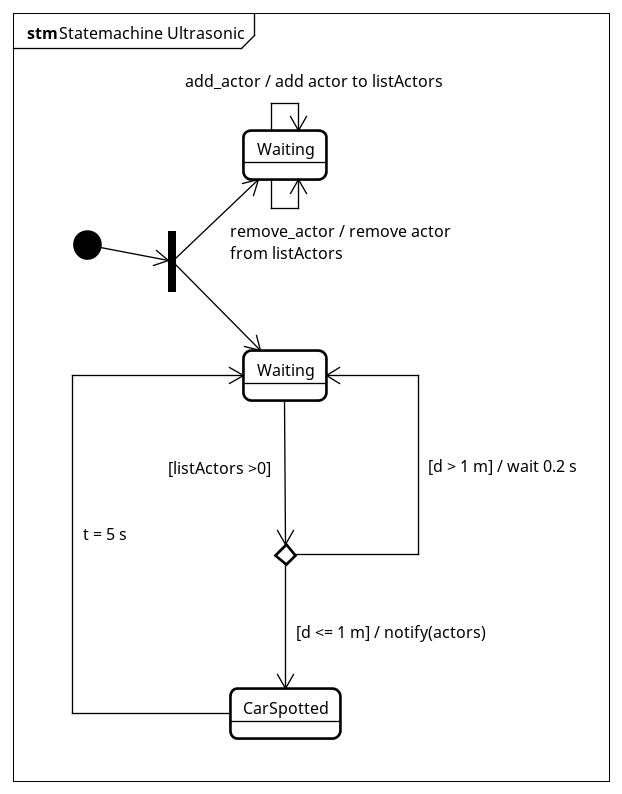
\includegraphics[scale=.75]{figure/Statemachine_Ultrasonic.png}
	\caption{Finished State Machine riguardante la parte di controllo presenza auto \label{FSM CAR}}
\end{figure}


\subsection{Cambiamento di stato dei lampioni}
Utilizzando il diagramma di sequenza in figura \ref{SD CAR} è stato rappresentato il cambio di stato da parte di due lampioni dal risparmio energetico alla piena potenza dopo la rilevazione di un'auto in transito.
Inizialmente i lampioni si trovano nello stato di risparmio energetico e viene effettuata una misurazione da parte del sensore di prossimità che restituisce la lettura rappresentata da 'd'.
In seguito viene eseguita una seconda lettura e questa volta la distanza rilevata si assume equivalga a meno di un metro, e quindi che sia stata rilevata un'automobile.
Per questo vengono notificati entrambi i lampioni, i quali, dopo un intervallo di tempo calcolato tramite la moltiplicazione tra una costante e il proprio id, passano in modalità piena potenza per permettere all'automobilista di percorrere la strada in sicurezza.

\begin{figure}[tbp]
	\centering
	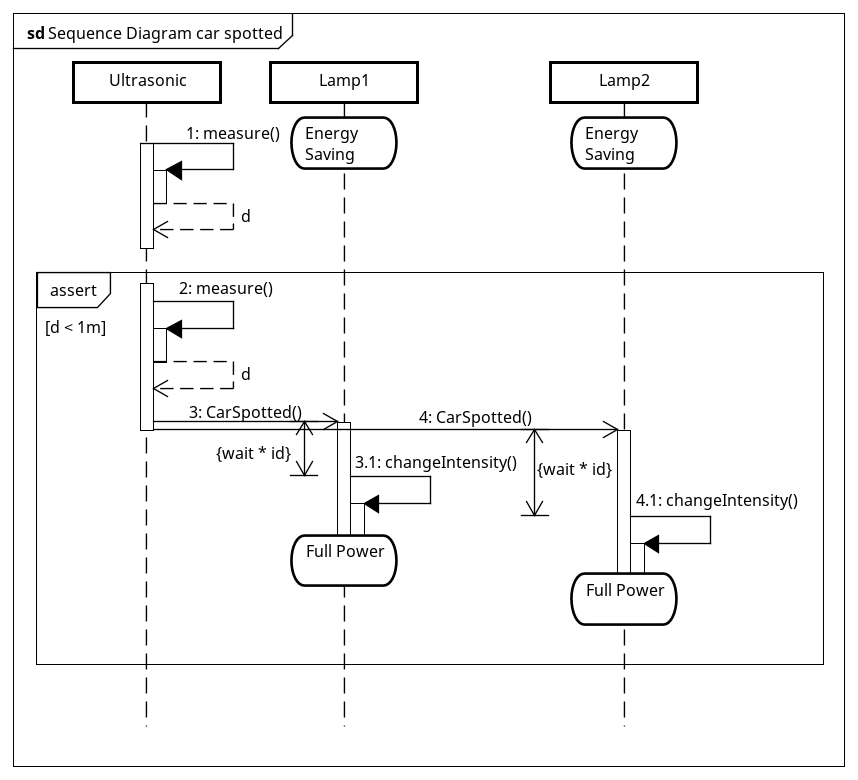
\includegraphics[scale=.59]{figure/Sequence_Diagram_car_spotted.png}
	\caption{Comunicazione tra il sensore ad ultrasuoni e i lampioni rappresentata tramite un Sequence Diagram \label{SD CAR}}
\end{figure}

\section{Controllo luminosità ambientale}
Questa parte si occupa di controllare l'intensità luminosa ambientale e di notificare i lampioni in modo che possano accendersi o spegnersi se il valore di luminosità sia maggiore o minore di una certa soglia impostata nelle loro policy.

\subsection{Architettura}

Per la rappresentazione dell'architettura è stato scelto di utilizzare una Finished State Machine.
In figura \ref{FSM PR} viene mostrato come inizialmente siano generati due thread concorrenti. Come per il caso del controllo della presenza di auto, anche qui un thread è responsabile della gestione della lista dei lampioni da notificare. Il secondo thread invece si occupa di eseguire la lettura dell'intensità luminosa e di notificare ogni lampione presente nella lista.
Il secondo thread parte dallo stato "waiting" ed esegue una lettura se la lista dei lampioni non è vuota. In seguito invia la lettura effettuata a tutti gli elementi della lista e aspetta nello stato "prMeasured" 10 secondi. Infine torna nello stato "waiting".


\begin{figure}[tbp]
	\centering
	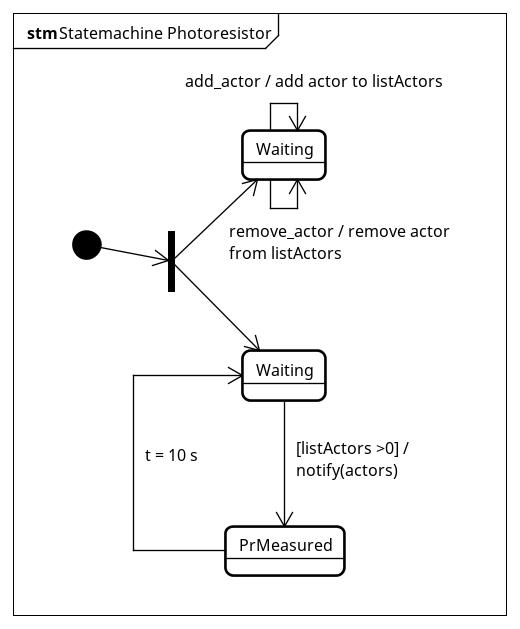
\includegraphics[scale=.8]{figure/Statemachine_Photoresistor.png}
	\caption{Finished State Machine riguardante la lettura della luminosità ambientale \label{FSM PR}}
\end{figure}
\newpage

\section{Web Server}
Il web server deve poter comunicare con i Raspberry Pi dislocati sul territorio per poter ottenere e modificare le impostazioni locali di ogni dispositivo.
Per questo scopo il web server si mette in comunicazione con i Raspberry utilizzando le loro interfacce (TODO: si chiamano interfacce?) REST.

\subsection{Diagramma di sequenza}
Come si può vedere in figura \ref{SD WEB} per la rappresentazione della comunicazione tra il web server e i Raspberry è stato utilizzato un diagramma di sequenza.
Nel primo esempio viene mostrata la richiesta da parte di un utente di ricevere le policy relative al lampione numero 1 da un determinato Raspberry.
Il web server utilizzando un url prestabilito effettua una GET. Il Raspberry ottiene le policy in formato json dal lampione 1 e restituisce tali informazioni al web server che successivamente le mostrerà all'utente.
Il secondo esempio è simile al primo con la differenza che in questo caso l'utente intende effettuare una modifica alla policy on del lampione 1. Quindi il web server questa volta invierà una POST al Raspberry di competenza, il quale notificherà del cambiamento il lampione coinvolto. Infine verrà mostrato all'utente l'esito di tale operazione.

\begin{figure}[tbp]
	\centering
	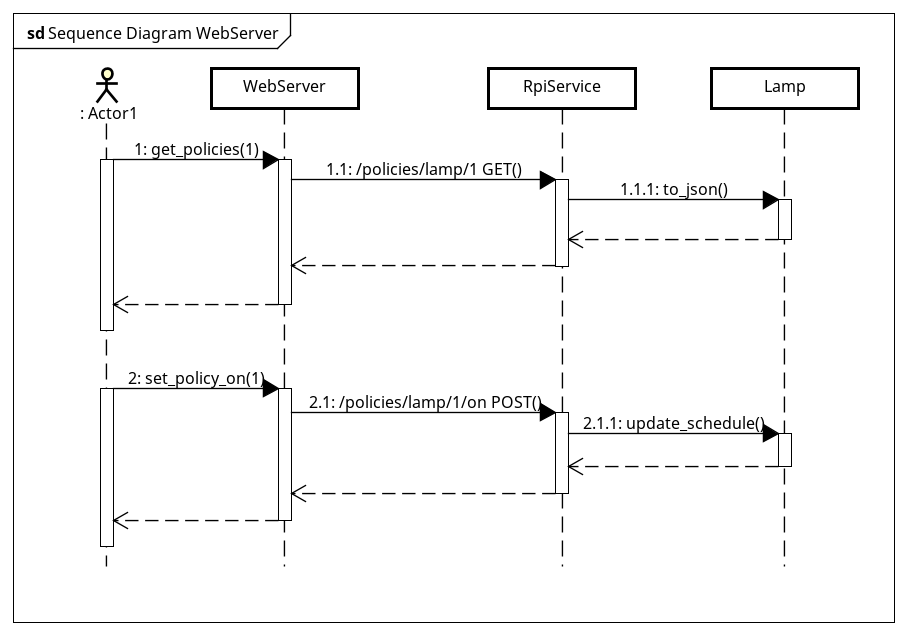
\includegraphics[scale=.55]{figure/Sequence_Diagram_WebServer.png}
	\caption{Sequence diagram per la comunicazione tra web server e Raspberry Pi \label{SD WEB}}
\end{figure}

